\documentclass[11pt]{article}
\usepackage{fullpage}
\usepackage{url}
\usepackage{amsmath, graphicx}
\begin{document}
\thispagestyle{empty}
\parindent 0pt
\vfill
\large

\begin{center}
\LARGE{\bf \textsf{CS246: Mining Massive Datasets}}\\ {\bf \textsf{Homework 3}}
\\*[4ex]
\end{center}

\section*{Answer to Question 1(a)}
The derivative wrt $R_{iu}$:
\begin{equation*}
\begin{aligned}
    \epsilon_{iu} = 2(R_{iu} -q_ip_u^{T})
\end{aligned}
\end{equation*}
The gradient wrt $q_i$:
\begin{equation*}
\begin{aligned}
    \frac{\partial E}{\partial q_i}
    = -2(R_{iu} -q_ip_u^{T})p_u + 2\lambda q_i
\end{aligned}
\end{equation*}
The gradient wrt $p_u$:
\begin{equation*}
\begin{aligned}
    \frac{\partial E}{\partial p_u}
    = -2(R_{iu} -q_ip_u^{T})q_i + 2\lambda p_u
\end{aligned}
\end{equation*}
When get rating $R_{ui}$, the stochastic gradient decent update for $q_i$:
\begin{equation}
q_{i}^{(t)} \leftarrow q_{i}^{(t-1)} - \mu[-2(R_{ui} -q_{i}^{(t-1)}p_{u}^{(t-1)^T})p_{u}^{(t-1)} + 2\lambda q_{i}^{t-1}]
\end{equation}
When get rating $R_{ui}$, The stochastic gradient decent update for $p_u$:
\begin{equation}
p_{u}^{(t)} \leftarrow p_{u}^{(t-1)} - \mu[-2(R_{ui} -q_{i}^{(t-1)}p_{u}^{(t-1)^T})q_{i}^{(t-1)} + 2\lambda p_{u}^{t-1}]
\end{equation}


\pagebreak[4]
\section*{Answer to Question 1(b)}
The error after 40 iteration is $54583.9$
\begin{figure}[h]
\center
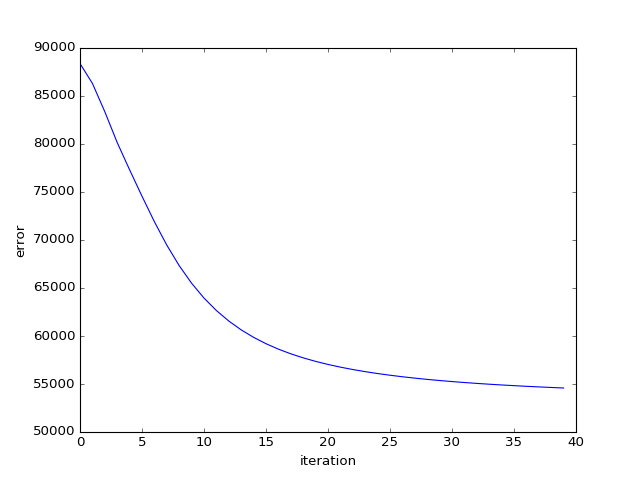
\includegraphics[scale=0.7]{iteration.png}
\caption{SGD converge, $\eta = 0.02$}
\end{figure}


\pagebreak[4]
\section*{Answer to Question 2(a)}
C1 and C2 will be merged together by centroid based merging.
This is due to the centroid of C1 is $0.73$,
the centroid of C2 is $0.93$ and the centroid of C3 is $1.2$.
C1 and C2 are much closer to each other.\\
\\
C2 and C3 will be merged together by closeset memeber based merging.
The most closeset point between C2 and C3 is only $0.02$ away. While C1 and C2 are $0.08$ away.\\
\\
Centroid based merging will behind two clusters
such that one of the clusters corresponds to the low risk of lung cancer and the other represents high risk.

\pagebreak[4]
\section*{Answer to Question 2(b)}
Centroid based merging is stable since when removing $P_6$, the outcome is still cluster C1 and C2 will be merged together.
While closed member based merging will merge C1 and C2 together instead of C2 and C3.
When $P_6$ is removed, closeset point between C2 and C3 is $0.09$ which is larger than $0.08$ the distance between C1 and C2.

\pagebreak[4]
\section*{Answer to Question 2(c)}
I would prefer using a stable merge strategy.
$5\%$ noise under unstable merging strategy can produce stochastically different result each time running the algorithm.
Therefore, I prefer a more stable merge strategy.\\
\\
The closeset member based merge only uses two points to decide the merge.
The noise will have a much larger impacts on closeset member based merge due to its small sample size.
While centroid based merge uses more points to make the decision, then it is less vulnerable to the noise.

\pagebreak[4]
\section*{Answer to Question 3(a)}
Take any two random nodes from $C_i$, since all the nodes from $C_i$ can be divided by $i$,
therefore, these two random nodes can be divided by $i$ as well. This means $i$ is their common factor and there exists an edge between them.
Then it is proved that all nodes from $C_i$ have edge between each other, whcih means $C_i$ is a clique.

\pagebreak[4]
\section*{Answer to Question 3(b)}
$C_i$ is a maximal clique if and only if $min(C_i) = i$ and $i$ should be a prime; also for any interger $k$ greater than $1$ either $ki \in C_i$ or $ki \geq 1000000$.\\
\\
Sufficient:\\
As proved in 3a, $C_i$ is a clique. If $i$ is a prime, it only has a factor of $1$ and itself. In order to be clique, all the elements in $C_i$ must be a multiplier of $i$.
Once $\forall c\in C_i$ and for any interger greater than $1$, $kc \in C_i$, then $C_i$ should include all the possible number.\\
\\
Necessary:\\
If $C_i$ is a maximal clique, it will definitely contain all the number that is a multiplier of $i$.
Then we need to justify that $i$ must be a prime. If $i$ is not a prime and $C_i$ is still a maximal clique, we can simply find a prime that is a divisor of $i$.
Obviously this divisor cannot be divided by $i$. Therefore, $i$ must be a prime.

\pagebreak[4]
\section*{Answer to Question 3(c)}
There can be more than 2 maximal clique.

\pagebreak[4]
\section*{Answer to Question 4(a)}
First proved
$$
|A(S)| \geq \frac{\epsilon}{1+\epsilon}|S|
$$
We can find that
$$
|E(S)| = \frac{1}{2}\sum_{i\in S}deg(i)
$$
Then,
$$
2|E(s)| = \sum_{i\in S}deg(i) \geq \sum_{i\in S/A(s)}deg(i)
$$
By eliminating subsets $A(S)$ the remaining elements should have degree at least $2(1+\epsilon)\rho(S)$:

\begin{equation*}
\begin{aligned}
2|E(s)| & \geq \sum_{i\in S/A(s)}deg(i)\\
& \geq (|S|-|A(S)|)2(1+\epsilon)\rho(S)\\
& = (|S|-|A(S)|)2(1+\epsilon)\frac{|E(S)|}{|S|}
\end{aligned}
\end{equation*}

Therefore,
$$
|S| \geq (1+\epsilon)(|S|-|A(S)|)
$$
$$
(1+\epsilon)|A(S)| \geq \epsilon|S|
$$
\begin{equation}
|A(S)| \geq \frac{\epsilon}{1+\epsilon}|S|
\end{equation}

If iteration starts with $n$ node, with $k$ iteration, there shoud be at most this much nodes left:
$$
\left(1 - \frac{\epsilon}{1+\epsilon}\right)^{k}n
$$
The iteration stops when the remaining node is less than 1:
$$
\left(1 - \frac{\epsilon}{1+\epsilon}\right)^{k}n \leq 1
$$
$$
\left(\frac{1}{1+\epsilon}\right)^k \leq 1/n
$$
Therefore, the maximal iteration step is:
\begin{equation}
k \leq \log_{1/(1+\epsilon)}^{1/n} = \log_{1+\epsilon}^{n}
\end{equation}


\pagebreak[4]
\section*{Answer to Question 4(b)}
Given $S^{*}$ is the densest subgraph, by taking away any nodes from it, its density can only decrease:
$$
\frac{\rho^{*}(G)|G|-deg_{S^{*}}(v)}{|G|-1} \leq \rho^{*}(G)
$$
Rearragne this, then have:
$$
\rho^{*}(G)|G|-deg_{S^{*}}(v) \leq \rho^{*}(G)|G| - \rho^{*}(G)
$$
\begin{equation}
\rho^{*}(G) \leq deg_{S^{*}}(v)
\end{equation}

If in the first iteration, there exists a node $v$, $v\in S^{*}\cap A(S)$, for $v$:
$$
2(1+\epsilon)\rho(S) \geq deg_{S}(v) \geq deg_{S^*}(v) \geq \rho^{*}(G)
$$

Therefore if at any iteration step with remaining set $S'$, eliminating a node belongs to $S^{*}$:
$$
\rho(S') \geq \frac{1}{2(1+\epsilon)}\rho^{*}(G)
$$
As we know $\rho(\tilde{S}) \geq \rho(S')$, therefore:
\begin{equation}
    \rho(\tilde{S}) \geq \frac{1}{2(1+\epsilon)}\rho^{*}(G)
\end{equation}

\pagebreak[4]
\begin{center}
\LARGE{\bf \textsf{Cover Sheet}} \\*[4ex]
\end{center}

\textbf{Assignment Submission } Fill in and include this cover sheet with each of your assignments. Assignments are due at 11:59pm. All students (SCPD and non-SCPD) must submit their homeworks via GradeScope (\url{http://www.gradescope.com}). Students can typeset or scan their homeworks. Make sure that you answer each question on a separate page. Students also need to upload their code at \url{http://snap.stanford.edu/submit}. Put all the code for a single question into a single file and upload it. Please do not put any code in your GradeScope submissions.
\\
\\
\textbf{Late Day Policy } Each student will have a total of {\em two} free late periods. {\em One late period expires at the start of each class.} (Homeworks are usually due on Thursdays, which means the first late periods expires on the following Tuesday.) Once these late periods are exhausted, any assignments turned in late will be penalized 50\% per late period. However, no assignment will be accepted more than {\em one} late period after its due date.
\\
\\
\textbf{Honor Code } We strongly encourage students to form study groups. Students may discuss and work on homework problems in groups. However, each student must write down their solutions independently i.e., each student must understand the solution well enough in order to reconstruct it by him/herself.  Students should clearly mention the names of all the other students who were part of their discussion group. Using code or solutions obtained from the web (github/google/previous year solutions etc.) is considered an honor code violation. We check all the submissions for plagiarism. We take the honor code very seriously and expect students to do the same.

\vfill
\vfill

{\Large
\textbf{Your name:} \hrulefill \\
\textbf{Email:} \underline{\hspace*{7cm}} \textbf{SUID:} \hrulefill\\*[2ex] }
Discussion Group (People with whom you discussed ideas used in your answers): \\\\\\
On-line or hardcopy documents used as part of your answers: \\\\\\
\vfill

\vfill

I acknowledge and accept the Honor Code.\\*[3ex]
\bigskip
\textit{(Signed)}\hrulefill
% If you are not printing this document out, just type your initials above

\vfill
\vfill

\end{document}

